% Options for packages loaded elsewhere
\PassOptionsToPackage{unicode}{hyperref}
\PassOptionsToPackage{hyphens}{url}
%
\documentclass[
]{book}
\usepackage{amsmath,amssymb}
\usepackage{iftex}
\ifPDFTeX
  \usepackage[T1]{fontenc}
  \usepackage[utf8]{inputenc}
  \usepackage{textcomp} % provide euro and other symbols
\else % if luatex or xetex
  \usepackage{unicode-math} % this also loads fontspec
  \defaultfontfeatures{Scale=MatchLowercase}
  \defaultfontfeatures[\rmfamily]{Ligatures=TeX,Scale=1}
\fi
\usepackage{lmodern}
\ifPDFTeX\else
  % xetex/luatex font selection
\fi
% Use upquote if available, for straight quotes in verbatim environments
\IfFileExists{upquote.sty}{\usepackage{upquote}}{}
\IfFileExists{microtype.sty}{% use microtype if available
  \usepackage[]{microtype}
  \UseMicrotypeSet[protrusion]{basicmath} % disable protrusion for tt fonts
}{}
\makeatletter
\@ifundefined{KOMAClassName}{% if non-KOMA class
  \IfFileExists{parskip.sty}{%
    \usepackage{parskip}
  }{% else
    \setlength{\parindent}{0pt}
    \setlength{\parskip}{6pt plus 2pt minus 1pt}}
}{% if KOMA class
  \KOMAoptions{parskip=half}}
\makeatother
\usepackage{xcolor}
\usepackage{longtable,booktabs,array}
\usepackage{calc} % for calculating minipage widths
% Correct order of tables after \paragraph or \subparagraph
\usepackage{etoolbox}
\makeatletter
\patchcmd\longtable{\par}{\if@noskipsec\mbox{}\fi\par}{}{}
\makeatother
% Allow footnotes in longtable head/foot
\IfFileExists{footnotehyper.sty}{\usepackage{footnotehyper}}{\usepackage{footnote}}
\makesavenoteenv{longtable}
\usepackage{graphicx}
\makeatletter
\def\maxwidth{\ifdim\Gin@nat@width>\linewidth\linewidth\else\Gin@nat@width\fi}
\def\maxheight{\ifdim\Gin@nat@height>\textheight\textheight\else\Gin@nat@height\fi}
\makeatother
% Scale images if necessary, so that they will not overflow the page
% margins by default, and it is still possible to overwrite the defaults
% using explicit options in \includegraphics[width, height, ...]{}
\setkeys{Gin}{width=\maxwidth,height=\maxheight,keepaspectratio}
% Set default figure placement to htbp
\makeatletter
\def\fps@figure{htbp}
\makeatother
\setlength{\emergencystretch}{3em} % prevent overfull lines
\providecommand{\tightlist}{%
  \setlength{\itemsep}{0pt}\setlength{\parskip}{0pt}}
\setcounter{secnumdepth}{5}
\usepackage{booktabs}
\ifLuaTeX
  \usepackage{selnolig}  % disable illegal ligatures
\fi
\usepackage[]{natbib}
\bibliographystyle{apalike}
\IfFileExists{bookmark.sty}{\usepackage{bookmark}}{\usepackage{hyperref}}
\IfFileExists{xurl.sty}{\usepackage{xurl}}{} % add URL line breaks if available
\urlstyle{same}
\hypersetup{
  pdftitle={Baltic Health Index Toolbox Manual},
  pdfauthor={Baltic Health Index Team},
  hidelinks,
  pdfcreator={LaTeX via pandoc}}

\title{Baltic Health Index Toolbox Manual}
\author{Baltic Health Index Team}
\date{2023-11-08}

\begin{document}
\maketitle

{
\setcounter{tocdepth}{1}
\tableofcontents
}
\hypertarget{welcome}{%
\chapter{Welcome}\label{welcome}}

Hi! \\
This manual is the Toolbox Manual for the Baltic Health Index (BHI).
It takes inspiration from the \href{http://ohi-science.org/toolbox-training/}{Ocean Health Index Toolbox Training} and it is adapted according to the unique features of the Baltic Sea.

The aim of this manual is to help you get ``on board'' with \href{http://ohi-science.org}{Ocean Health Index (OHI)} methods and practices as you lead your own independent OHI assessment (OHI\textsuperscript{+}) in the Baltic Sea.

The OHI process has 4 steps: \textbf{Learn}, \textbf{Plan}, \textbf{Conduct}, and \textbf{Inform}. These steps are overlapping and iterative: as you plan your assessment you will continue to learn, as you conduct your assessment you will need to modify your plan and keep team members and stakeholders informed.

\begin{center}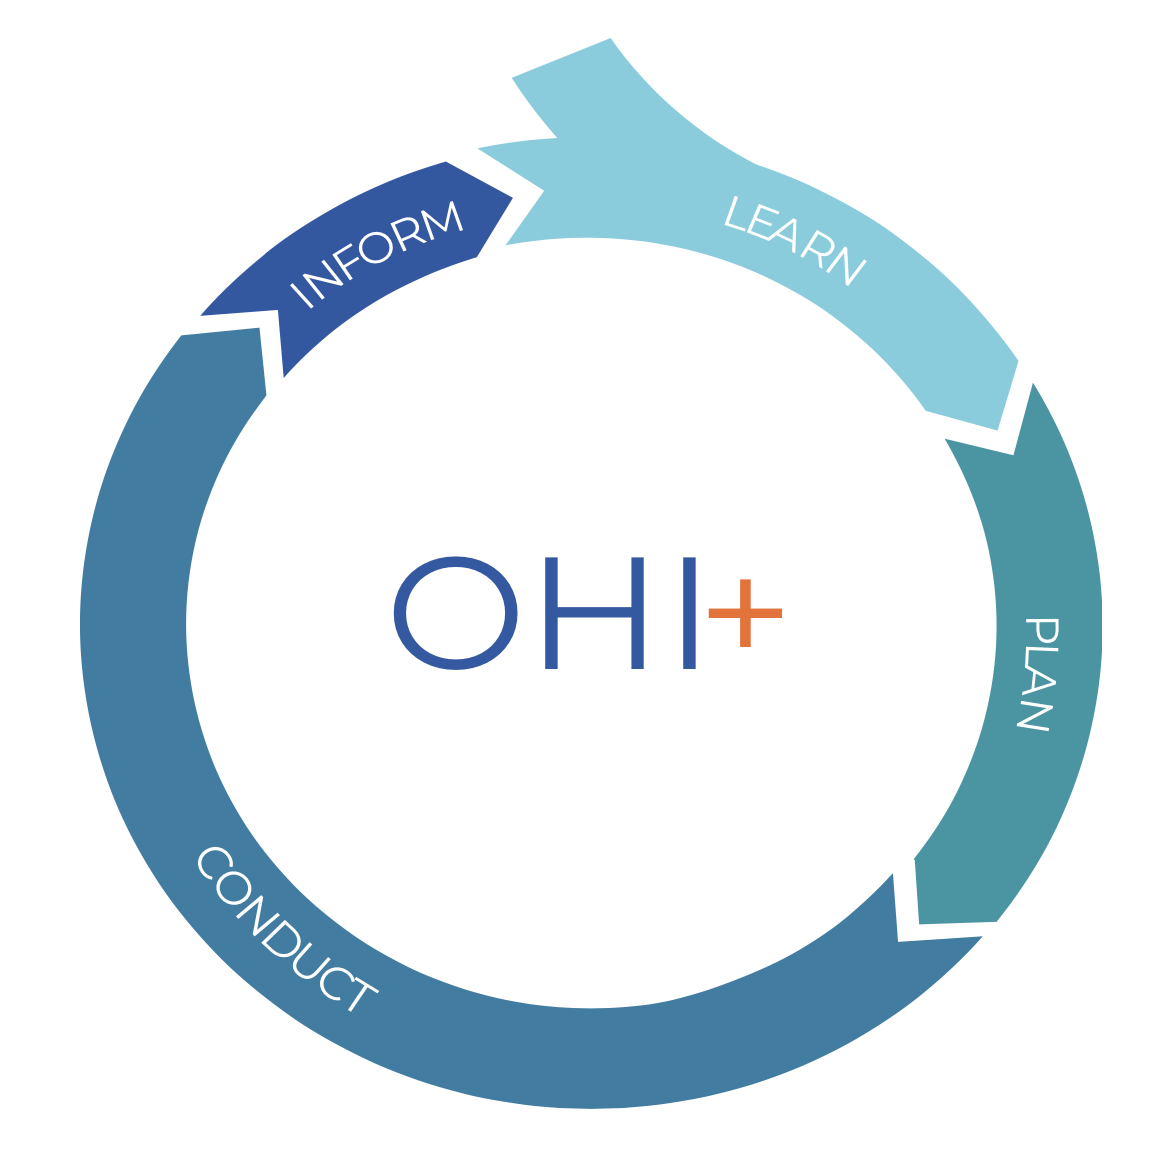
\includegraphics[width=500px]{_book/_main_files/figure-html/ohi-process} \end{center}

\hypertarget{what-is-the-baltic-health-index}{%
\chapter{What is the Baltic Health Index?}\label{what-is-the-baltic-health-index}}

\begin{center}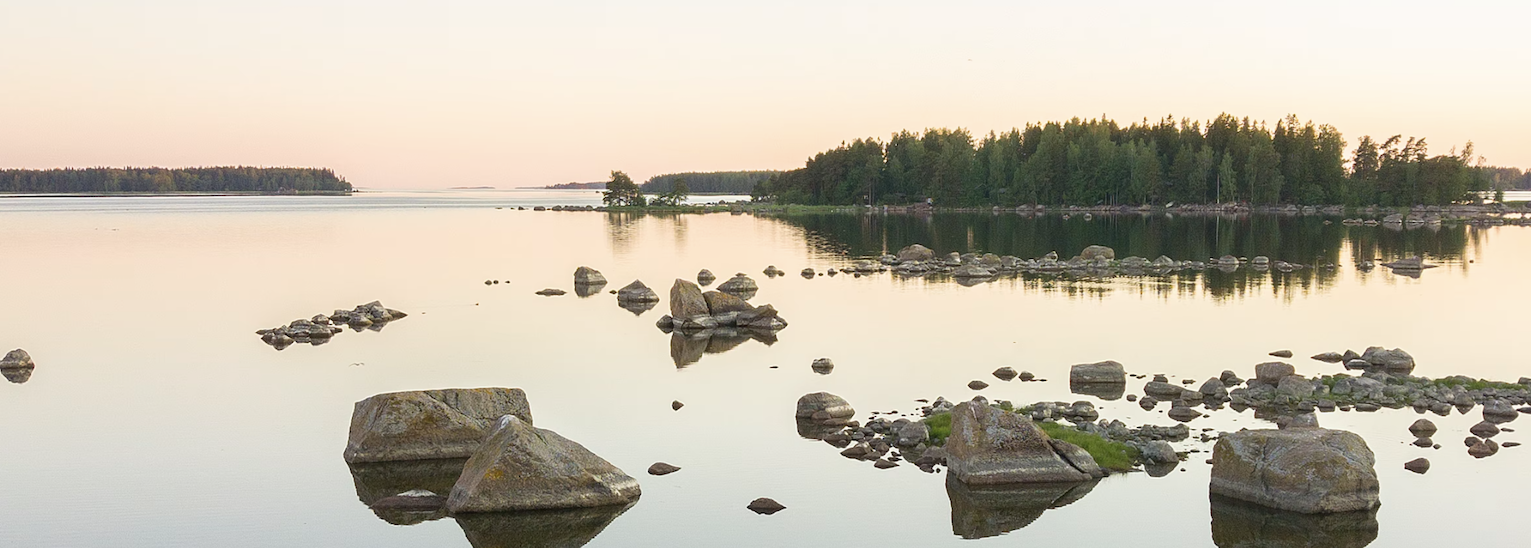
\includegraphics[width=800px]{_book/_main_files/figure-html/banner-image-rocks} \end{center}

The \textbf{Baltic Health Index (BHI)} is a comprehensive assessment tool that evaluates a suite of goals that sustainably deliver benefits to humans in the Baltic Sea. It can also be tailored to identify and capture important factors in different contexts.

\hypertarget{open-science}{%
\section*{Open Science}\label{open-science}}
\addcontentsline{toc}{section}{Open Science}

The biggest motivation of the Ocean Health Index is to use the best available science, data, methods, and tools to inform marine management. OHI assessments use collaborative open software so that they are transparent and reproducible.

\hypertarget{what-other-ohi-assessments-have-done}{%
\section*{\texorpdfstring{What other OHI\textsuperscript{+} assessments have done?}{What other OHI+ assessments have done?}}\label{what-other-ohi-assessments-have-done}}
\addcontentsline{toc}{section}{What other OHI\textsuperscript{+} assessments have done?}

What other OHI local assessments (aka OHI+) have been done, where?

\begin{itemize}
\tightlist
\item
  \url{https://oceanhealthindex.org/ohi+/conduct/}
\item
  \href{https://github.com/OHI-Norway/}{Norway}
\item
  \href{https://www.ohi.sustainable-seas.org/}{Cornwall/Southwest England}
\item
  \href{https://github.com/OHI-Science/ohi-canada}{Canada}
\item
  \href{https://github.com/OHI-Science/ohibc}{Canada-British Columbia}
\item
  \href{http://ohi-science.org/bali/}{Bali}
\item
  \href{http://ohi-science.org/mhi/}{Hawaii}
\item
  \href{https://github.com/OHI-Science/arc}{Arctic}
\end{itemize}

\begin{figure}

{\centering 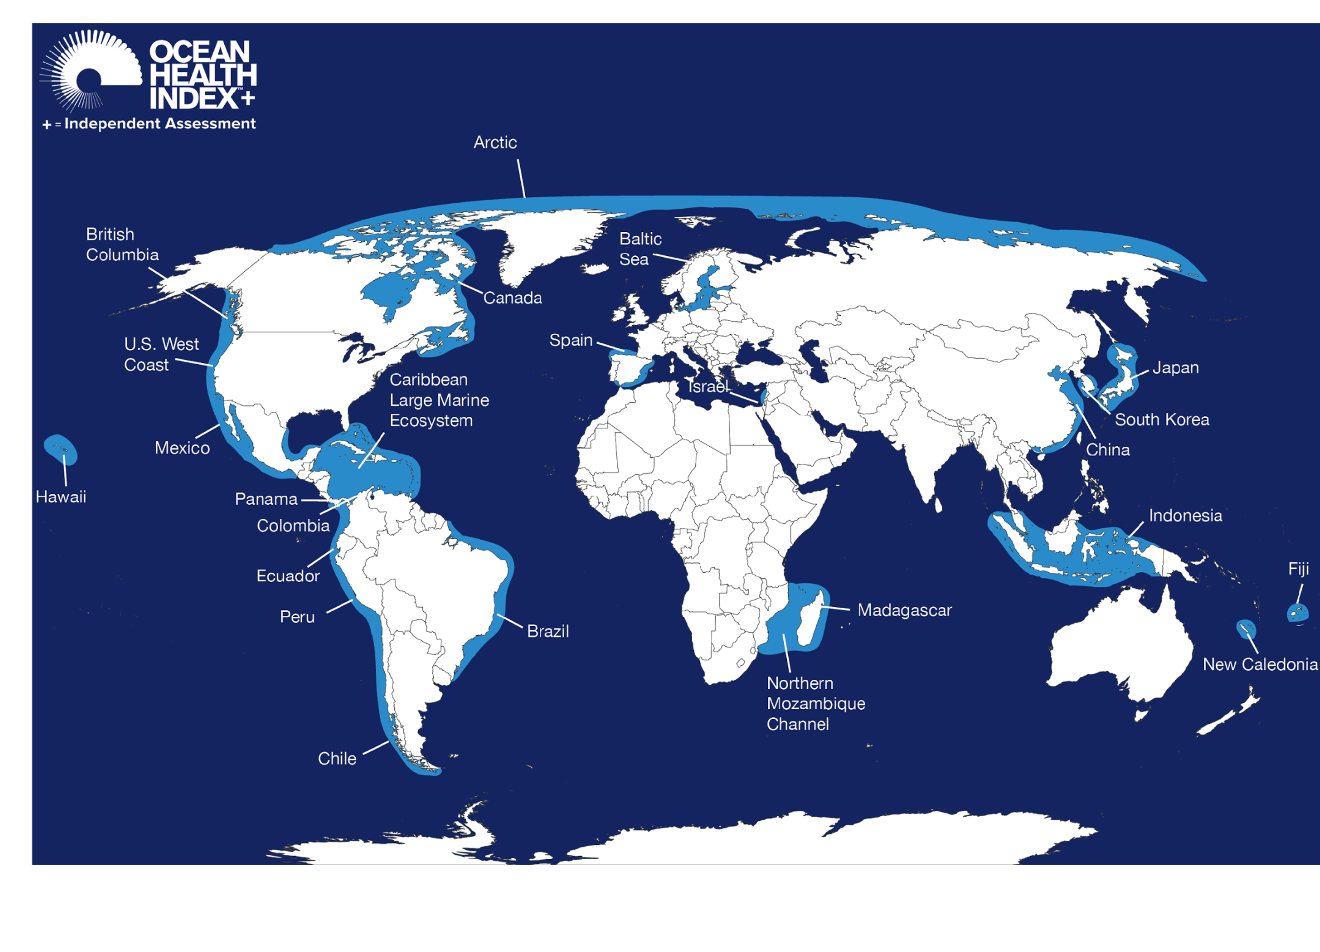
\includegraphics[width=800px]{_book/_main_files/figure-html/ohi+_map} 

}

\caption{OHI local assessments around the world.}\label{fig:unnamed-chunk-3}
\end{figure}

\hypertarget{get-set-up-with-r-rstudio-git-github}{%
\chapter{Get set up with R, Rstudio, Git \& Github}\label{get-set-up-with-r-rstudio-git-github}}

\begin{center}
\includegraphics[width=800px]{_book/_main_files/figure-html/tech-toolkit} \end{center}

Making OHI\textsuperscript{+} assessments in the Baltic Sea requires coding and using data science software.
You can learn this in a fun and empowering way!

In the OHI \href{http://ohi-science.org/data-science-training/}{Open Data Science} training book you will learn a reproducible workflow with R, RStudio, Git, and GitHub.

But before the training, please make sure you have done the following:

\begin{enumerate}
\def\labelenumi{\arabic{enumi})}
\tightlist
\item
  Download and install up-to-date versions of:

  \begin{itemize}
  \tightlist
  \item
    \textbf{R}: \url{https://cloud.r-project.org}
  \item
    \textbf{RStudio}: \url{http://www.rstudio.com/download}
  \item
    \textbf{Git}: \url{https://git-scm.com/downloads} \emph{Note: open the download and follow normal install procedures on your computer but you won't see any software installed when you're done}
  \end{itemize}
\item
  Create a \textbf{GitHub account}: \url{https://github.com} \emph{Note: shorter names can identify you are better, and use your work email!}
\item
  Get comfortable: if you're not in a physical workshop, be set up with two screens if possible. You will be following along in RStudio on your own computer while also watching a virtual training or following this tutorial on your own.
\end{enumerate}

\hypertarget{further-trainings-and-learning}{%
\section*{Further Trainings and Learning}\label{further-trainings-and-learning}}
\addcontentsline{toc}{section}{Further Trainings and Learning}

\begin{itemize}
\tightlist
\item
  \href{https://youtube.com/playlist?list=PLX7J3qtjcll_4s2oaKHuWdRdBMJz7tBAU\&si=NIoCjH-AuOM-rWkI}{OHI Intro to Data Science Training Youtube series}, where you will learn more about collaborative tools.
\item
  \href{https://swirlstats.com/}{Swirl}, where you can learn R programming and data science interactively, at your own pace, and right in the R console!
\item
  \href{https://stat545.com}{Stat545}, where you will explore, groom, visualize, and analyze data, make all of that reproducible, reusable, and shareable using R.
\item
  \href{https://r4ds.hadley.nz}{R for Data Science}, a book that will teach you how to do data science with R.
\item
  \href{https://openscapes.github.io/series/core-lessons/github/github-issues.html}{Improving collaboration with Github}, where you learn to use Github for communication and project management through GitHub Issues.
\item
  \href{https://learning.nceas.ucsb.edu/2021-11-RRCourse/}{Reproducible Research Techniques},to help researchers with good data science skills, share data with the scientific community effectively and efficiently, and benefit from the re-use of their data by others.
\end{itemize}

\hypertarget{underlying-theory-concepts-and-framework}{%
\chapter{Underlying theory, concepts and framework}\label{underlying-theory-concepts-and-framework}}

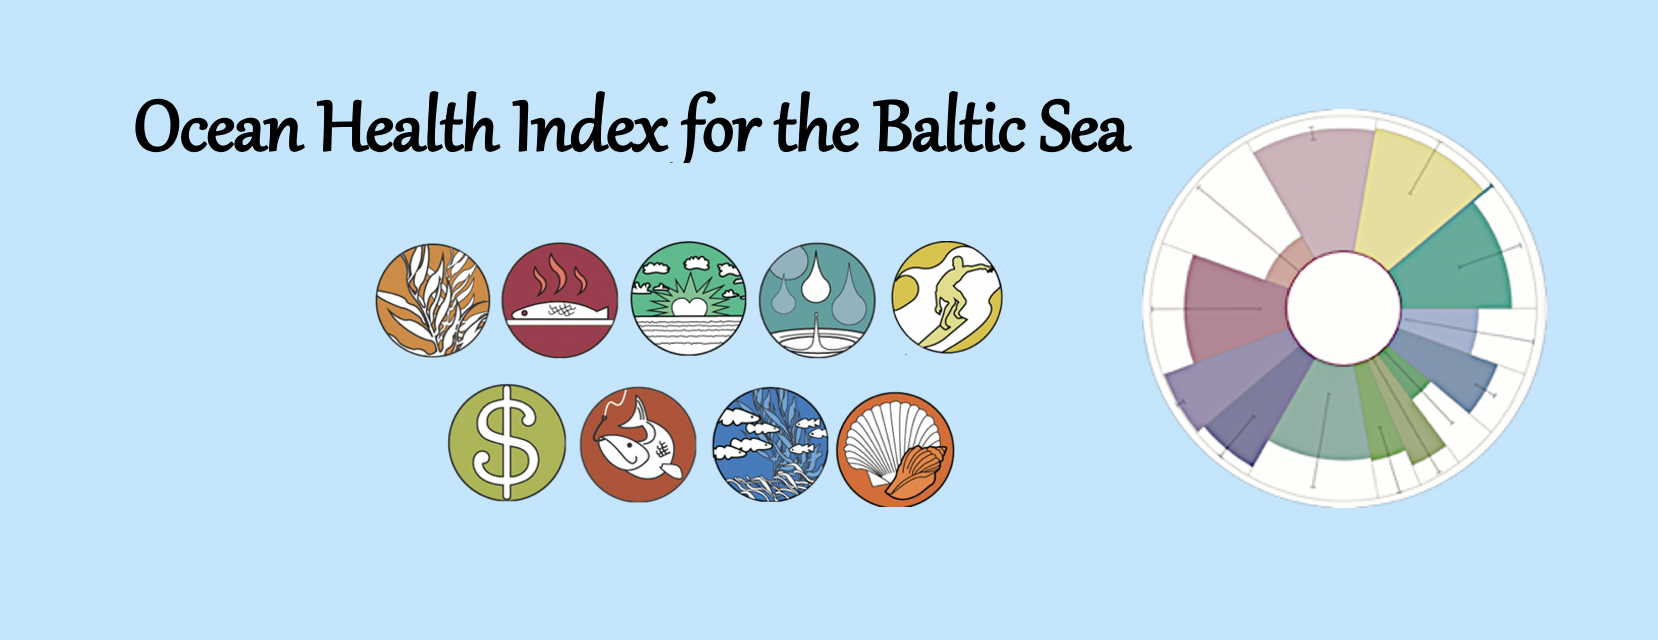
\includegraphics[width=800px]{_book/_main_files/figure-html/twitter_pic}

The OHI framework categorizes \textbf{goals} and \textbf{sub-goals} representing ocean-derived benefits to people.

When creating the framework, scientists, economists, and sociologists review existing studies of what people want and expect from the ocean and then group them these categories called `goals.'

Each goal is scored on the delivery of specific benefits with respect to a sustainable target. A goal is given a score of 100 if its benefits are maximized without compromising the ocean's ability to deliver those benefits in the future. Lower scores indicate that more benefits could be gained or that current methods are harming the delivery of future benefits.

\hypertarget{dimensions-of-the-index}{%
\section*{Dimensions of the Index}\label{dimensions-of-the-index}}
\addcontentsline{toc}{section}{Dimensions of the Index}

Goal Scores are based on several components: current status, likely future status, trend, pressures, and resilience.

To calculate each Goal Score we average the \textbf{Present Status} and \textbf{Likely Future Status}:

\begin{itemize}
\item
  \textbf{PRESENT STATUS} is a goal's current value compared to its reference point, resulting in a score from 0 to 100.
\item
  \textbf{LIKELY FUTURE STATUS} is the predicted status score five years into the future (once again, on a scale from 0 to 100), which is estimated by adjusting the current status score by 3 variables:

  \begin{itemize}
  \tightlist
  \item
    \textbf{TREND} indicates how fast the system is moving in a given direction, like velocity (rate of change)
  \item
    \textbf{PRESSURES} which are the ecological and social factors that decrease a goal's status.
  \item
    \textbf{RESILIENCE} which are ecological factors and social initiatives (policies, laws, etc.) that mitigate the pressures acting on a goal.
  \end{itemize}
\end{itemize}

\begin{figure}

{\centering 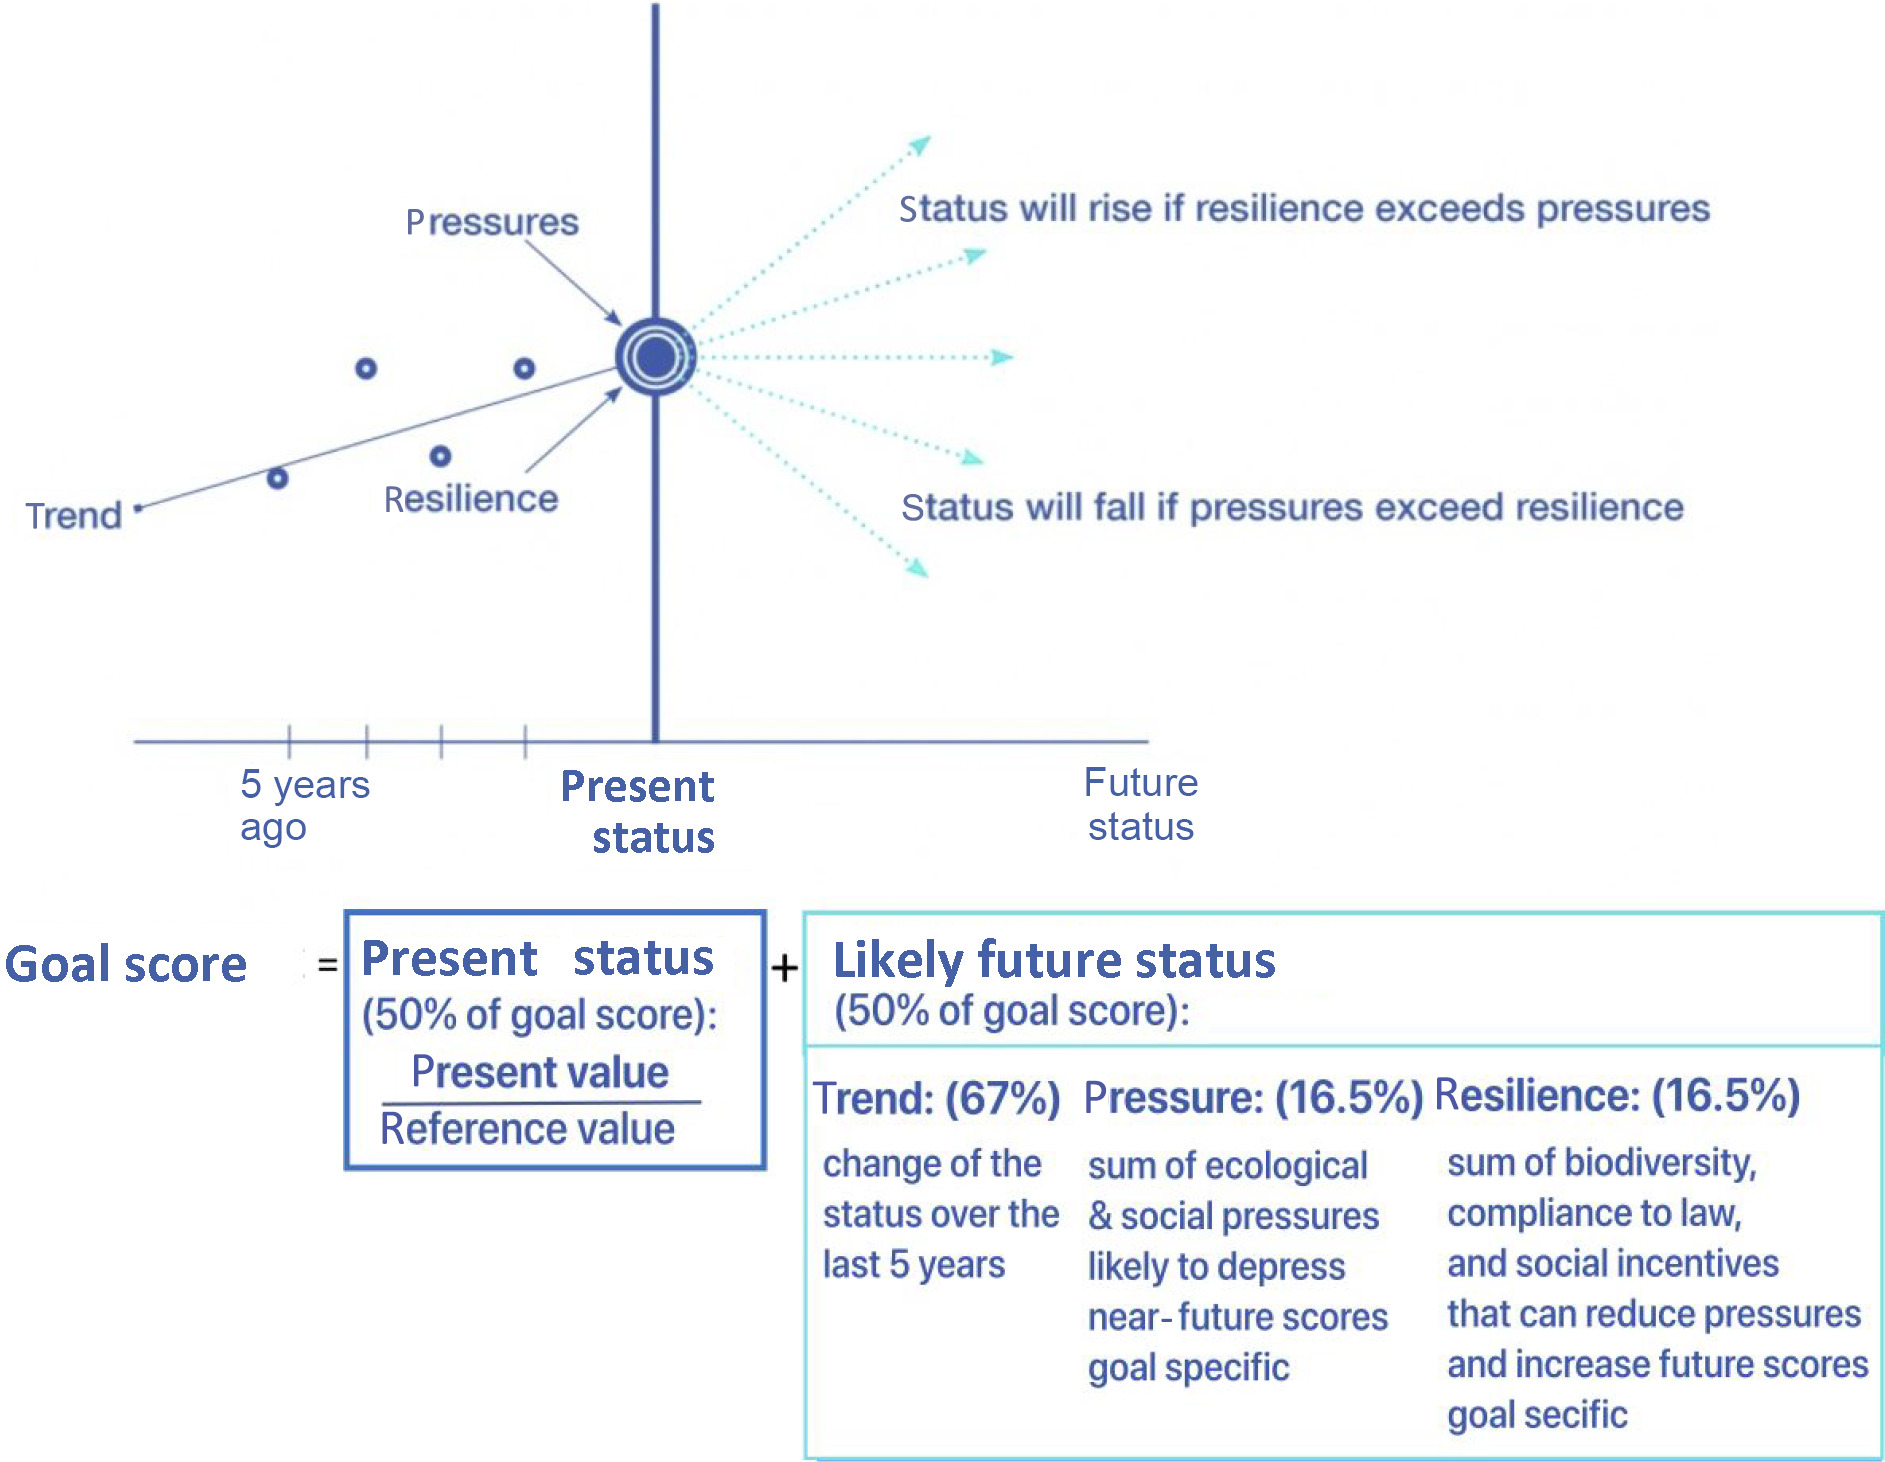
\includegraphics[width=800px]{_book/_main_files/figure-html/ohi-dimensions} 

}

\caption{OHI representation of how each goal score is calculated}\label{fig:unnamed-chunk-6}
\end{figure}

\begin{center}\rule{0.5\linewidth}{0.5pt}\end{center}

\hypertarget{glossary}{%
\section*{Glossary}\label{glossary}}
\addcontentsline{toc}{section}{Glossary}

\begin{itemize}
\tightlist
\item
  \textbf{Region's Index Score}: the average of its goal scores. Goal scores are weighted equally in regional and global assessments, but independent assessments could weight them differently depending on local conditions and values.
\item
  \ldots{}
\end{itemize}

\hypertarget{bhi-local-get-started}{%
\chapter{BHI-local -- Get Started!}\label{bhi-local-get-started}}

The OHI\textsuperscript{+} is a step-by-step standardized process with an adaptive capacity to meet local necessities and needs, which leads to the creation of effective integrated management approaches for the ocean and coastal ecosystems.
Planning a BHI\textsuperscript{+} assessment requires identifying the \textbf{needs} and \textbf{spatial areas} of the assessment, establishing \textbf{objectives} and a \textbf{timeline of activities}, determining \textbf{necessary resources} (human and financial), and aligning the assessment process with existing efforts and initiatives.

The following are key ingredients when creating a local assessment from scratch.

\hypertarget{a-qualified-technical-team}{%
\section{A qualified technical team}\label{a-qualified-technical-team}}

A \textbf{core team} that is very knowledgeable about the BHI framework and process, and \textbf{`Goal-keepers'} that are experts in specific BHI\textsuperscript{+} goals to help develop the best models, access information, identify pressures and resilience measures, and set reference points, through in-person meetings, workshops, and remote communication.

\begin{center}
\includegraphics[width=800px]{_book/_main_files/figure-html/workshop-unsplash-photo-by-patrick-perkins} \end{center}

\hypertarget{policy-and-management-interest}{%
\section{Policy and Management Interest}\label{policy-and-management-interest}}

BHI\textsuperscript{+} assessments can be used to \textbf{inform} government policies to \textbf{improve} ocean health. This is most effective if there is interest and engagement from policy makers and ongoing communication during the BHI\textsuperscript{+} process, so the resulting index is better tailored to measure features and impacts of concern, targeted by \textbf{management actions}.

\hypertarget{funding}{%
\section{Funding}\label{funding}}

The costs to complete BHI\textsuperscript{+} assessments vary depending on the local context, and the first will need more investment than subsequent assessments. Financial support is needed for a management and technical team, workshops and meetings (including travel), communication, policy engagement, and operating costs. Therefore, \textbf{securing funding} is an important component to satisfactorily complete assessments and building institutional memory. The development of a local proposal or strategic action plan that details a timeline of activities, including the resources needed to accomplish them, is encouraged.

\hypertarget{data-and-indicators}{%
\section{Data and Indicators}\label{data-and-indicators}}

BHI\textsuperscript{+} assessments require gathering existing data and indicators to \textbf{represent relevant BHI\textsuperscript{+} goals}, and the pressures and resilience actions interacting with those goals. Information can come from environmental, social, and economic sources.
It takes time to identify, gather, and process these data and indicators, and accessing the \textbf{best available information} is of highest importance. It is important to communicate where data gaps exist and which data are not ideal to be used; \textbf{identifying missing information} helps highlight areas for future improvement (see also this \href{https://docs.google.com/spreadsheets/d/1f-vwUrQHrMs7cjhChuK2YnlbkE_5kQ6AgGwyV2eJ1vA/edit\#gid=1485393150}{OHI Data Planner} to help you organize your thinking around the data available and how it could be used in your BHI\textsuperscript{+} assessment).

\begin{center}\rule{0.5\linewidth}{0.5pt}\end{center}

\hypertarget{steps}{%
\section*{Steps}\label{steps}}
\addcontentsline{toc}{section}{Steps}

BHI\textsuperscript{+} assessments use the same framework as the BHI assessments, but allow for exploration of variables influencing ocean health at the \textbf{smaller scales} where policy and management decisions are made. Goal models and targets are created using higher resolution data, indicators, and priorities, which produce scores \textbf{better reflecting local realities}. This enables scientists, managers, policy makers, and the public to better and more holistically understand, track, and communicate the status of local marine ecosystems, and to \textbf{design strategic management actions} to improve overall ocean health.

\hypertarget{creating-a-vision-whats-the-purpose-of-this-bhi-assessment}{%
\subsection*{\texorpdfstring{1) Creating a Vision: What's the purpose of this BHI\textsuperscript{+} assessment?}{1) Creating a Vision: What's the purpose of this BHI+ assessment?}}\label{creating-a-vision-whats-the-purpose-of-this-bhi-assessment}}
\addcontentsline{toc}{subsection}{1) Creating a Vision: What's the purpose of this BHI\textsuperscript{+} assessment?}

Creating the Index is not the end goal: it is merely a process toward the true end goal -- \textbf{achieving improved ocean health}. Establishing a common vision and determining early in the process how the findings will be used and by whom, makes the final goal clear to the greater community (as well as to stakeholders and participants). Establishing a vision will help identify outstanding important issues that may need to be addressed later on. For example:

\begin{itemize}
\tightlist
\item
  What are the existing stakeholder problems, needs, and interests that need to be addressed? Are there conflicting uses of ocean and coastal resources?
\item
  Is the objective to use the findings to reform policies and/or improve practices?
\item
  Are there any specific management priorities established through government mandates, private sector initiatives, and/or international treaty obligations that would especially benefit from an Index assessment? Are there any special management needs?
\end{itemize}

\hypertarget{identifying-local-characteristics-and-priorities}{%
\subsection*{2) Identifying local characteristics and priorities}\label{identifying-local-characteristics-and-priorities}}
\addcontentsline{toc}{subsection}{2) Identifying local characteristics and priorities}

Identifying local characteristics and priorities for ocean health is crucial for determining the goals to be assessed. Examples of goals used in the BHI are: \emph{Artisanal Fishing Opportunities}, \emph{Biodiversity}, \emph{Carbon Storage}, \emph{Clean Waters}, \emph{Food Provision}, \emph{Livelihoods and Economies}, \emph{Natural Products}, \emph{Sense of Place}, and \emph{Tourism}. You may remove the goals that are irrelevant or add new ones that are relevant to your local area. Understanding which goals and ocean benefits are important in the proposed study area, and what threats or possible changes might be affecting the sustainable delivery of those benefits is essential when identifying goals. Also, it can be important to establish which priorities are most and least influential (e.g.~use of goal weightings when combining all goals).

\hypertarget{defining-spatial-areas}{%
\subsection*{3) Defining spatial areas}\label{defining-spatial-areas}}
\addcontentsline{toc}{subsection}{3) Defining spatial areas}

Defining spatial regions and boundaries is essential for BHI\textsuperscript{+} assessments. Moreover, balancing the importance of biophysical boundaries with management boundaries is important when creating a local assessment, as often these do not exactly match up. Further, the scale of decision-making need to match with the scale of data availability.

\hypertarget{identifying-indicators-and-data}{%
\subsection*{4) Identifying indicators and data}\label{identifying-indicators-and-data}}
\addcontentsline{toc}{subsection}{4) Identifying indicators and data}

When we define goals, we need to be thinking about indicators that help us measure those goals. How to represent goals and set spatial boundaries is guided by the type and quality of data that are available. There are practical and philosophical reasons for including or excluding data, including relevance to ocean health, accessibility, quality, existence of a reference point, and spatial and temporal scales. Ideally, data must be available for every region within the study area and for the five most-recent years to calculate the recent trend. For some goals, where temporal reference points are desirable, longer time series are preferable. An important question to reflect on when identifying indicators is: \textbf{What should the goal capture?}

\hypertarget{establishing-reference-points}{%
\subsection*{5) Establishing reference points}\label{establishing-reference-points}}
\addcontentsline{toc}{subsection}{5) Establishing reference points}

Establishing sustainable reference points as explicit benchmarks using \textbf{SMART} criteria is key: \textbf{S}pecific (to the management objective), \textbf{M}easurable, \textbf{A}mbitious, \textbf{R}ealistic, and \textbf{T}ime-bound (Perrings et al.~2010, 2011). Reference points are set specifically to the local context to capture stakeholder priorities such that goal scores reflect progress towards achieving those targets, and future assessments can serve as a measure of the effectiveness of management and policy interventions. Reference points should, in fact, \textbf{align with management targets} established on a predetermined timeline.

\hypertarget{establishing-pressures-and-resilience-measures}{%
\subsection*{6) Establishing Pressures and Resilience measures}\label{establishing-pressures-and-resilience-measures}}
\addcontentsline{toc}{subsection}{6) Establishing Pressures and Resilience measures}

The BHI core framework has two fundamental requirements for calculating scores:

\begin{itemize}
\tightlist
\item
  It requires information on the \textbf{status} and \textbf{trend} for each goal and a wide range of \textbf{pressures} (negative influences) and \textbf{resilience} (positive influences) measures that will likely affect each goal status in the near future (Halpern et al., 2012);
\item
  Input information and the goals themselves must have an explicit benchmark or \textbf{`reference point'} to which they are compared (Samhouri et al., 2012), which enables goals to be scored on a dimensionless scale from 0 to 100, where a score of 100 represents full delivery of the goal as defined by fully meeting the explicit benchmark.
\end{itemize}

It is important to identify the pressures that affect the sea in the study area, and also which resilience measures, such as relevant environmental laws, could counteract those pressures. Ideally, every pressure with an identified strong impact should have a corresponding resilience measure.

\hypertarget{establishing-communications-and-outreach-efforts}{%
\subsection*{7) Establishing communications and outreach efforts}\label{establishing-communications-and-outreach-efforts}}
\addcontentsline{toc}{subsection}{7) Establishing communications and outreach efforts}

BHI\textsuperscript{+} assessments result in numeric scores which can be interpreted and communicated to many audiences. These scores enable comparisons between goals, across
assessment areas, and through time when assessments are repeated with the same methods. Such comparisons can help local managers to make decisions based on the best available science by identifying geographic and thematic priorities, altering the allocation of resources, and tracking management performance over time. Along with final scores and methods, it is important to transparently describe successes and challenges of the process (including information, uncertainty and knowledge gaps), as these can help to \textbf{prioritize policy decisions} and can also make future assessments more efficient.

\begin{figure}

{\centering 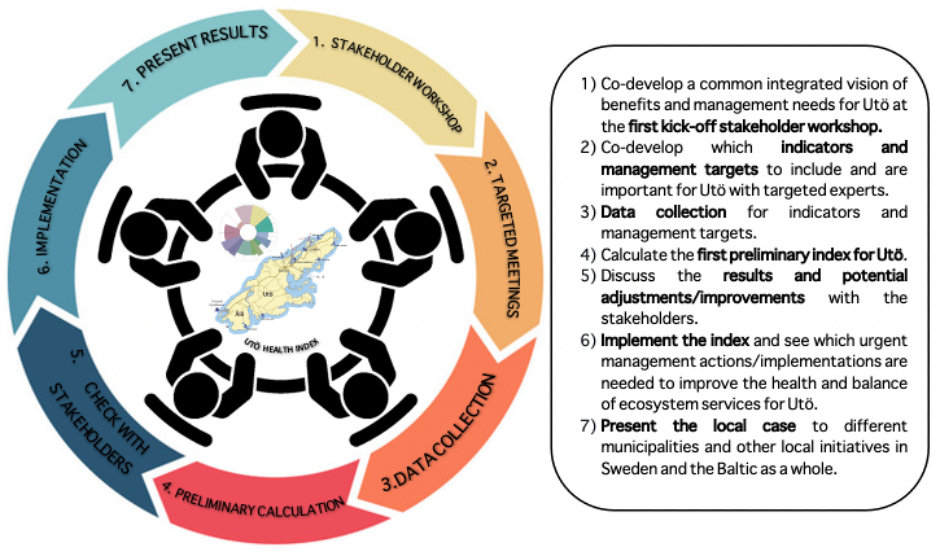
\includegraphics[width=800px]{_book/_main_files/figure-html/development-process} 

}

\caption{Schematic illustration showing the development process for the proposed Utö Health Index, as an example of a local case applying the BHI^+^ framework}\label{fig:unnamed-chunk-8}
\end{figure}

\hypertarget{data-management-for-bhi-local}{%
\section{Data management for BHI-local}\label{data-management-for-bhi-local}}

\emph{This will be expanded with more content soon!}

\hypertarget{the-process-of-preparing-data-for-the-index}{%
\section{The Process of Preparing data for the Index}\label{the-process-of-preparing-data-for-the-index}}

\emph{This will be expanded with more content soon!}

\hypertarget{calculating-the-index-scores-and-making-flowerplots}{%
\section{Calculating the Index Scores and making Flowerplots}\label{calculating-the-index-scores-and-making-flowerplots}}

\emph{This will be expanded with more content soon!}

\begin{center}\rule{0.5\linewidth}{0.5pt}\end{center}

\hypertarget{r-playground}{%
\chapter{R Playground!}\label{r-playground}}

\begin{enumerate}
\def\labelenumi{\arabic{enumi})}
\tightlist
\item
  Score calculation + Flowerplots
\item
  Add exercises with dummy data to explore the flowerplot function and let people play with it (try to find an `R playground', like MyBinder, sololearn, etc.)
\end{enumerate}

\hypertarget{further-readings-and-learnings}{%
\section*{Further Readings and Learnings}\label{further-readings-and-learnings}}
\addcontentsline{toc}{section}{Further Readings and Learnings}

\begin{itemize}
\item
  \href{https://www.nature.com/articles/s41559-017-0160}{Better science in less time}
\item
  \href{http://ohi-science.org/onboarding/}{Ocean Health Index Onboarding}, a higher-level overview of what the OHI is and how to start thinking about it with your team, and also where you can explore the 4 OHI process steps in more details.
\item
  \href{https://ohi-science.org/toolbox-training/index.html}{Ocean Health Index Toolbox Training}, which can train you to prepare for and use the OHI Toolbox (Conduct Phase).
\item
  \href{https://oceanhealthindex.org/resources/tools/}{More OHI Resources}
\item
  \href{https://ohi-science.org/news/goal-forward-approach}{What makes OHI stand out in the sea of environmental indicators? (Seifert 2018)}: It is a goal-forward approach.
\item
  \href{https://ohi-science.org/news/three-lessons-global}{Three Lessons for Using the Global Ocean Health Index to Assess Local Oceans (Seifert 2019)}: ``Three interrelated things seem to stand out: include the right people from the start, fit the framework to the place, and align with existing regional efforts.''
\item
  \href{https://esajournals.onlinelibrary.wiley.com/doi/full/10.1890/ES11-00366.1}{Sea sick? Setting targets to assess ocean health and ecosystem services}
\item
  \href{https://peerj.com/articles/1503/}{Best practices for assessing ocean health in multiple contexts using tailorable frameworks}
\end{itemize}

Xie, Yihui. 2023. Bookdown: Authoring Books and Technical Documents with r Markdown. \url{https://github.com/rstudio/bookdown}.
``Ocean Health Index. 2015. Ocean Health Index Toolbox Manual {[}2021{]}. National Center for Ecological Analysis and Synthesis, University of California, Santa Barbara. Available at: \url{http://ohi-science.org/manual}'

  \bibliography{book.bib,packages.bib}

\end{document}
